\documentclass[a4paper,14pt]{extreport}

% packages to support Cyrillic fonts, needed to write abstracts
\usepackage[T2A]{fontenc} 
\usepackage[utf8]{inputenc} 
\usepackage[russian,english]{babel}
\usepackage{csquotes}
\usepackage{listings}

% usual packages
\usepackage[left=30mm, right=25mm, top=20mm, bottom=25mm]{geometry}
\usepackage{graphicx} % to add figures
\graphicspath{{figures/}}

\usepackage{hyperref} % to add clickable contents menu

\usepackage[style=numeric]{biblatex}
\addbibresource{bibliography.bib}

\usepackage{blindtext}

% the following three definitions are to be changed by student
\def\myauthor{Niyara Muradova, Yernar Aimagambetov} % author
\def\mycoach{Ardak Shalkarbay-uly} % coach, adviser etc.
\def\mytitle{Popularization and development of blood donation platform} % title
%\def\mydegree{Bachelor in Computer Systems and Software}
%\def\mydegreecode{5B070400}
\def\mydegree{Bachelor in Information Systems}
\def\mydegreecode{6B061001}

% preamble ends here
\begin{document}
    % don't touch these two lines :)
    \begin{titlepage}
\begin{center}
\large
Ministry of Education and Science of the Republic of Kazakhstan

Suleyman Demirel University

\vspace{1cm}
\begin{figure}[h]
    \centering
    
\includegraphics[scale=0.5]{sdu_only}
\end{figure}

\vspace{2cm}
\Large
\myauthor

\vspace{1cm}
\Large
\textbf{\mytitle}

\vspace{1cm}
\large
A thesis submitted for the degree of

\mydegree

(degree code: \mydegreecode)

\vfill
Kaskelen, 2018

\end{center}
\end{titlepage}
    \newpage
\pagestyle{empty}

\begin{center}
\large
Ministry of Education and Science of the Republic of Kazakhstan

Suleyman Demirel University

Faculty of Engineering and Natural Sciences

\vspace{2cm}
\textbf{\mytitle}

\vspace{1cm}
\large
A thesis submitted for the degree of

\mydegree

(degree code: \mydegreecode)

\vspace{2cm}
Author: \textbf{\myauthor}

\vspace{2cm}
Supervisor: \textbf{\mycoach}

\vspace{2cm}
Dean of the faculty:

\textbf{Ph.D. Andrey Bogdanchikov}


\vfill
Kaskelen, 2021
\end{center}

    
    % edit abstracts
    \newpage
\pagestyle{plain}

\begin{center}
    \Large
    \textbf{Abstract}
    \setlength{\parindent}{15mm}
\end{center}
\par
Whilst the technology and medication methods develop in the field of medicine in Kazakhstan, people are forgetting about basic needs of healthcare. The continuous growth of blood needs and lack of blood donors leads us to serious difficulties such as shortage of blood required for blood transfusion and surgeons. The blood donation centers provide all of the required services to people in order to perform on a high level. But, as we can see, the improvements on the inside of the system are not leading to better results.
\par
The hope is that new vision to donation will bring equitable access not only to currently active donors but will attract other layers of people. New opportunities that are offered as a reward system will improve current situation and could enhance level of social happiness.
\par
Preliminary result on alpha-testing of the application are enough to provide stable base for further development not only in the blood donation field but also in other situations that require people's participation as donors. Additionally, we discuss close relationship between government, private companies and regular people in general so as to show how active cooperation can solve a lot of social problems as well.

    \newpage
\pagestyle{plain}

{\selectlanguage{russian}
\begin{center}
    \Large
    \textbf{Аңдатпа}
    \setlength{\parindent}{15mm}
\end{center}
\par
Қазақстанда емдеу технологиялары мен әдістері медицина саласында дамып жатқанда, адамдар денсаулық сақтаудың негізгі қажеттіліктерін ұмытып кетеді. Қан қажеттіліктерінің үнемі өсуі және қан донорларының жетіспеушілігі бізді қан құю мен хирургтар үшін қажет қанның жетіспеушілігі сияқты үлкен қиындықтарға алып келеді. Қан тапсыру орталықтары адамдарға жоғары деңгейде жұмыс істеу үшін барлық қажетті қызметтерді ұсынады. Бірақ, көріп отырғанымыздай, жүйенің ішіндегі жақсартулар жақсы нәтиже бермейді.
\par
Біз жаңа көрінісі донорлық қамтамасыз етеді және әділ қолжетімділігі ғана емес, қолданыстағы қазіргі уақытта донор емес, тартады басқа қабаттар адамдар.Сыйақы жүйесі ретінде ұсынылатын жаңа мүмкіндіктер қазіргі жағдайды жақсартады және әлеуметтік бақыт деңгейін жоғарылатуы мүмкін.
\par
Қосымшаның альфа-тестілеуінің алдын-ала нәтижелері қан тапсыру саласында ғана емес, сонымен қатар адамдардың донор ретінде қатысуын талап ететін басқа да жағдайларда одан әрі дамуы үшін тұрақты базаны қамтамасыз ету үшін жеткілікті. Сонымен қатар,біз белсенді ынтымақтастықтың көптеген әлеуметтік мәселелерді қалай шеше алатындығын көрсету үшін Үкімет, жеке компаниялар және жалпы қарапайым адамдар арасындағы тығыз қарым-қатынасты талқылаймыз.
}
    \newpage
\pagestyle{plain}

{\selectlanguage{russian}
\begin{center}
    \Large
    \textbf{Аннотация}
\end{center}
\par
В процессе развития новых технологий и методов медикаментозного лечения в медицине Казахстана, большинство людей забывают о базовых нуждах системы здравоохранения страны. Беспрерывный рост необходимости донорской крови и отсутсвие необходимого количества доноров приводят к серьезным сложностям в переливании крови и операциях. Центры крови на сегодняшний день предоставляют профессиональное обслуживание и функционируют на высшем уровне. Но, как мы можем наблюдать, улучшения внутри системы не ведут к позитивной динамике роста количества доноров.
\par
Новый взгляд на донорство предоставит равноправные условия как и для существующих активных доноров так и для новых привлеченных людей. Новые возможности, которые предлагаются в виде системы поощрений и достижений улучшат и стабилизируют текущую ситуация, а также повлияют на рост социального благополучя населения.
\par
Предварительные результаты тестирования системы на данном этапе достаточны для формирования устойчивой базы для дальнейшего развития проекта. Это обратит внимание не только на донорство крови, но и на другие сферы медицины, где необходимо участие людей как доноров. А также мы рассматриваем возможность близких взаимосвязей между государством, частными компаниями и обычными людьми, которая показывает как кооперативность и активная работа вместе помогает разрешению социальных проблем в целом.
}
    \tableofcontents
    
    % edit your chapters
    \begin{center}
    \setlength{\parindent}{15mm}
\end{center}
\chapter{Introduction}\label{ch:intro}
%these sections are optional, up-to the author
\section{Motivation}
\par
Blood transfusion is an extremely important process which saves millions of lives. But, the need and an actual number of donations are not currently balanced in Kazakhstan. 
\par
The reason for this may be absence of marketing and advertising of blood donation and no interest from the younger people to donate. Our project does all of the research and provides optimal solution in order to improve current situation in blood donation.
\par
Blood transfusion is an extremely important process which saves millions of lives. But, the need and an actual number of donations are not currently balanced in Kazakhstan. The actual reason for this may be absence of marketing and advertising of blood donation and no interest from the younger people to donate. Our project does all of the research and provides optimal solution in order to improve current situation in blood donation.
\par
According to World Health Organization, in general we need at least 20 blood donations per 1000 people. But in Kazakhstan the number of donations decreases every year and by 2021 we have only 14.7 blood donations. This leads to lack of blood and a lot of problems when we come to solving emergency situations. Decreasing numbers, no interest in population drives to develop strong community of blood donors.

\section{Aims and Objectives}
\par
The main goal is to increase number of donations firstly to a standard of World Health Organization and then even exceed the amount in order to create sustainable social balance in donation.
\par
By developing one platform for people to track their donations and receive valuable achievements, this will help attracting people to solving the real problem of current lack of blood in Kazakhstan. The recruitment system and marketing strategies will support the development of the 'Donor project' so that it won't be a one time interest, but a continuous and integrated system.
\par
At the Donor Project, we want prepared donors and in the right amount to come to blood centers every day. But this is a difficult and complex task. We are engaged in the correct donation of blood, that is, we are promoting this cause because we want, first of all, to help those in need of blood. But in order to realize and interest potential donors, we use the free main idea - Privileges. They include healthcare facilities and introduce people to a completely new possibility of receiving expensive medical diagnostic just by a blood donation.
\par
Working with government and private companies of healthcare in our country would have a positive impact on our society in general. Our project will attract new people and will integrate key partners existing.
\par
As a first step it is required to connect locally one city, so then we can scale up our online platform and connect other cities. The system doesn't require a lot of manipulations in order to scale, so the process will be easy and fast-forward if we have needed resources such as access to local healthcare organization's data.

\section{Thesis Outline}
The first chapter is \nameref{ch:intro} chapter. It is this one that you are currently reading. It gives insight into the work done. In Chapter \ref{ch:A} we review design system research and marketing strategies that were developed and used for the project. Chapter \ref{ch:B} is describing the solution to the problem and physical representation of online platform which was developed using popular frameworks and Object Oriented Language. And in \nameref{ch:concl} chapter we review our project as an ecosystem and share the results of the whole development process
    \chapter{Designing the methods and UX/UI research}\label{ch:A}
\section{General description}
\par
Actually, UX design sphere consists of some constituent elements like design usability, accessibility, comfortability, design system performance and testing. In this thesis I would talk about some of them like visual concepts, usability and in common design. Exactly, such thoughts about behavior and understanding of the user on web pages should be noted, which is very important in comfort for people. The process on the part of the user is very important here, since the project is intended for people of all ages and the research will help in the further implementation of the project. 
\par
For a good design to make a product befit, designers learn from their users how to do it using a variety of techniques and techniques in the UX industry. It is unique for each project.
\par
The project was not easy, the task was to create a website that will serve as an entrance to the world of donation, which includes completely different content that distinguishes it from all others, the one and only. My task was to implement a new design for desktop and mobile versions of the website to make it adaptive.
\par
A design system was used to superimpose interactions within the project, reference point and structure. Naturally, the project is clean from scratch, so the best solution was to make a list of all the different templates, colors, text styles and patterns that we use in our design \cite{eyal}. We started experimenting with some visual patterns like initial UI elements, layouts. The creation of various concepts and chose the most promising ones. 
\par
The usage of the principles of atomic design allowed to develop not only attracting interface, but also a system that is logically structured. As mentioned earlier, we started with some particles like colors, fonts, shapes. Moving on to atoms, buttons, inputs, containers and pagination from scratch of the construction is a method of designing a good usable interface. Finally, we made up the molecules - the search field, date-address pickers, navigation bars, side menus and organisms - lists, registration containers. Due to this, we were able to prepare templates for element pages -  our own UI kit system which has unique style and independent logic. 


\section{Design development and processing}
\par
When creating a project from scratch, the first idea and the process itself started from the main step - thinking \cite{eyal}. Thinking about the design began with drawing on a piece of paper. We had a few thoughts on how to implement the 'Donor project' design. The most important thing at that moment was to write down all the thoughts, even if they were good or bad. The general ideas were already established when we were stating the problems of current donation process and having collected it all into one we could begin working on further development of the idea, depending on our main aims and goals, such as simple interface but good logical construction. (see Figure \ref{fig:main})
\begin{figure}[h]
    \centering
    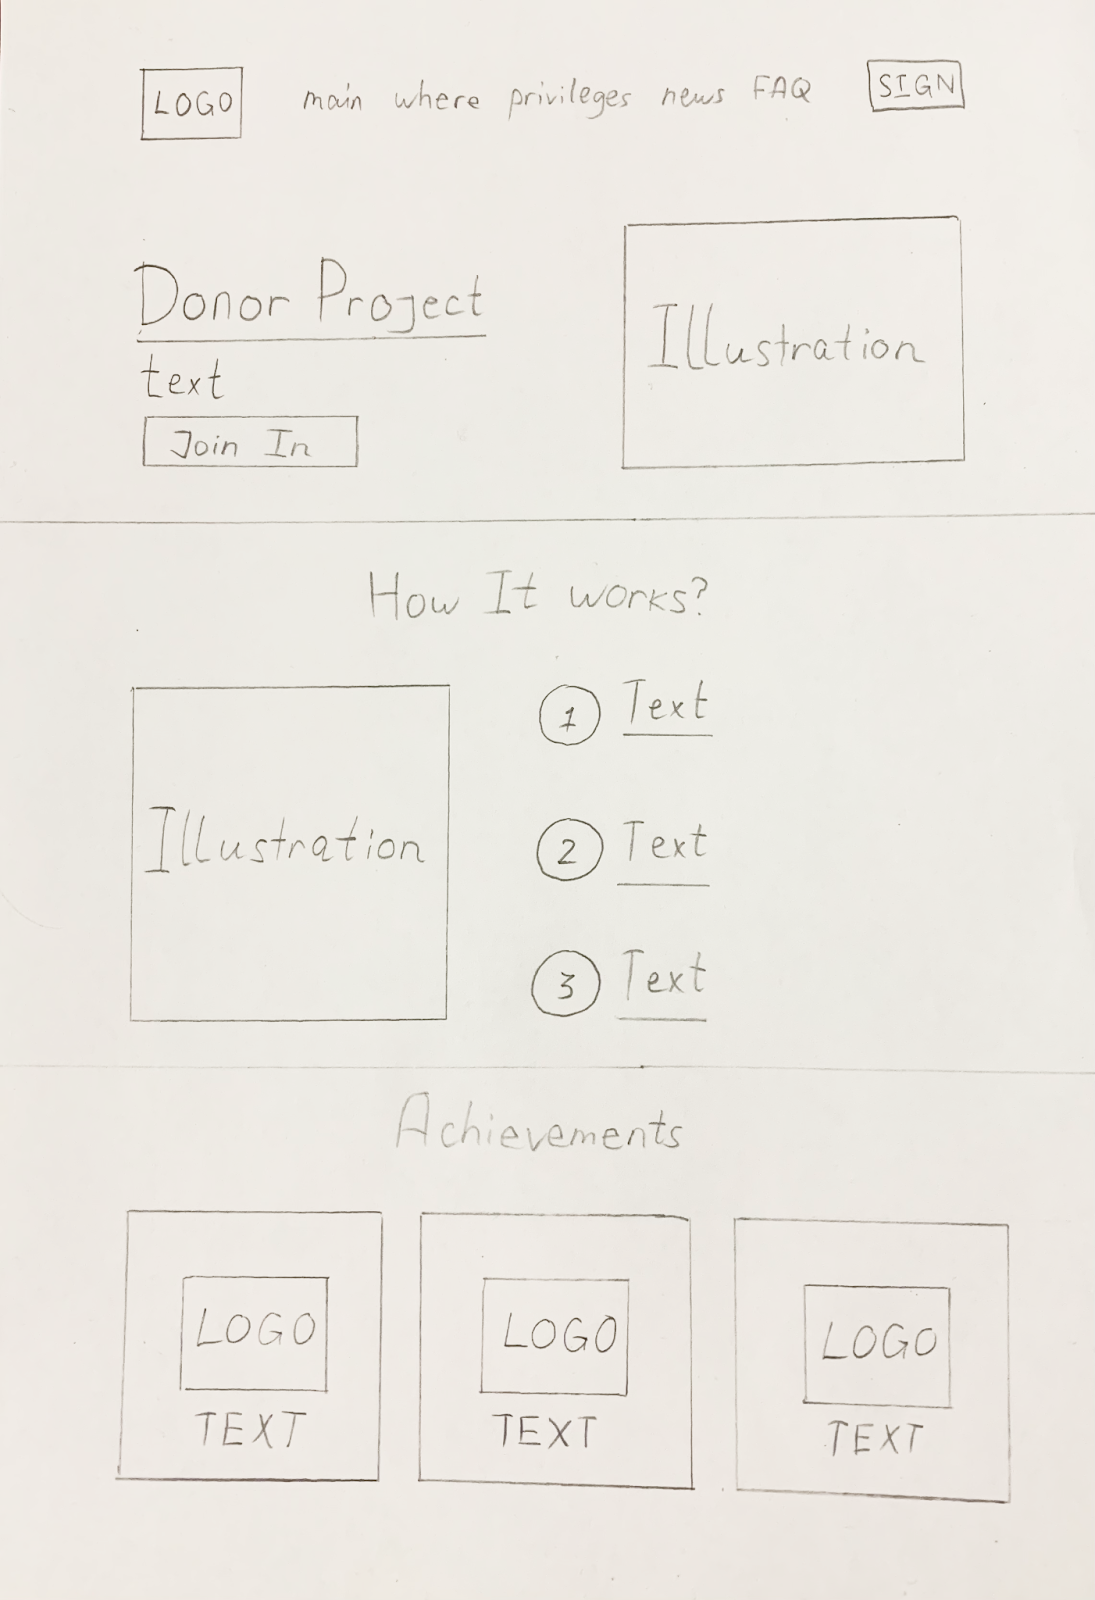
\includegraphics[scale=0.18]{figures/1.png}
    \caption{Sketch of the Main Page}
    \label{fig:main}
\end{figure}
To integrate, firstly researches were made on websites for competitive-promoting companies that are related to our market, looking at their designing and analyzing the idea behind it we got  more familiar with the donation industry. This gave a better understanding of how the pages on the donation site should look like. Writing down and memorizing best and bad practice became handy in the further design of the project and using other people's experience helped to develop better system \cite{martinez}. 
\par
Almost all sites that were used for research had main pages such as: a profile page, a question and answer page, a contact page.
After long deliberation over the pages that the 'Donor project' will have, the decision came to the general idea: Home, Where to donate blood, privileges, and FAQ. They served as the main pages in our header which conduct as a map of the website that will be developed.
\par
The name of the project and its description are in the first place. This is used on almost every site to show the user what the company is.
After the name of the company, the decision to present the company in the section how it works and the section footer.
Potential clients usually want to see the result of the company's work and what they are capable of \cite{martinez}. In this case, clients are potential donors of different ages. Therefore, the best solution is to provide the client with all the information about the project and what it represents. (see Figure \ref{fig:profilesketch})
\begin{figure}[h]
    \centering
    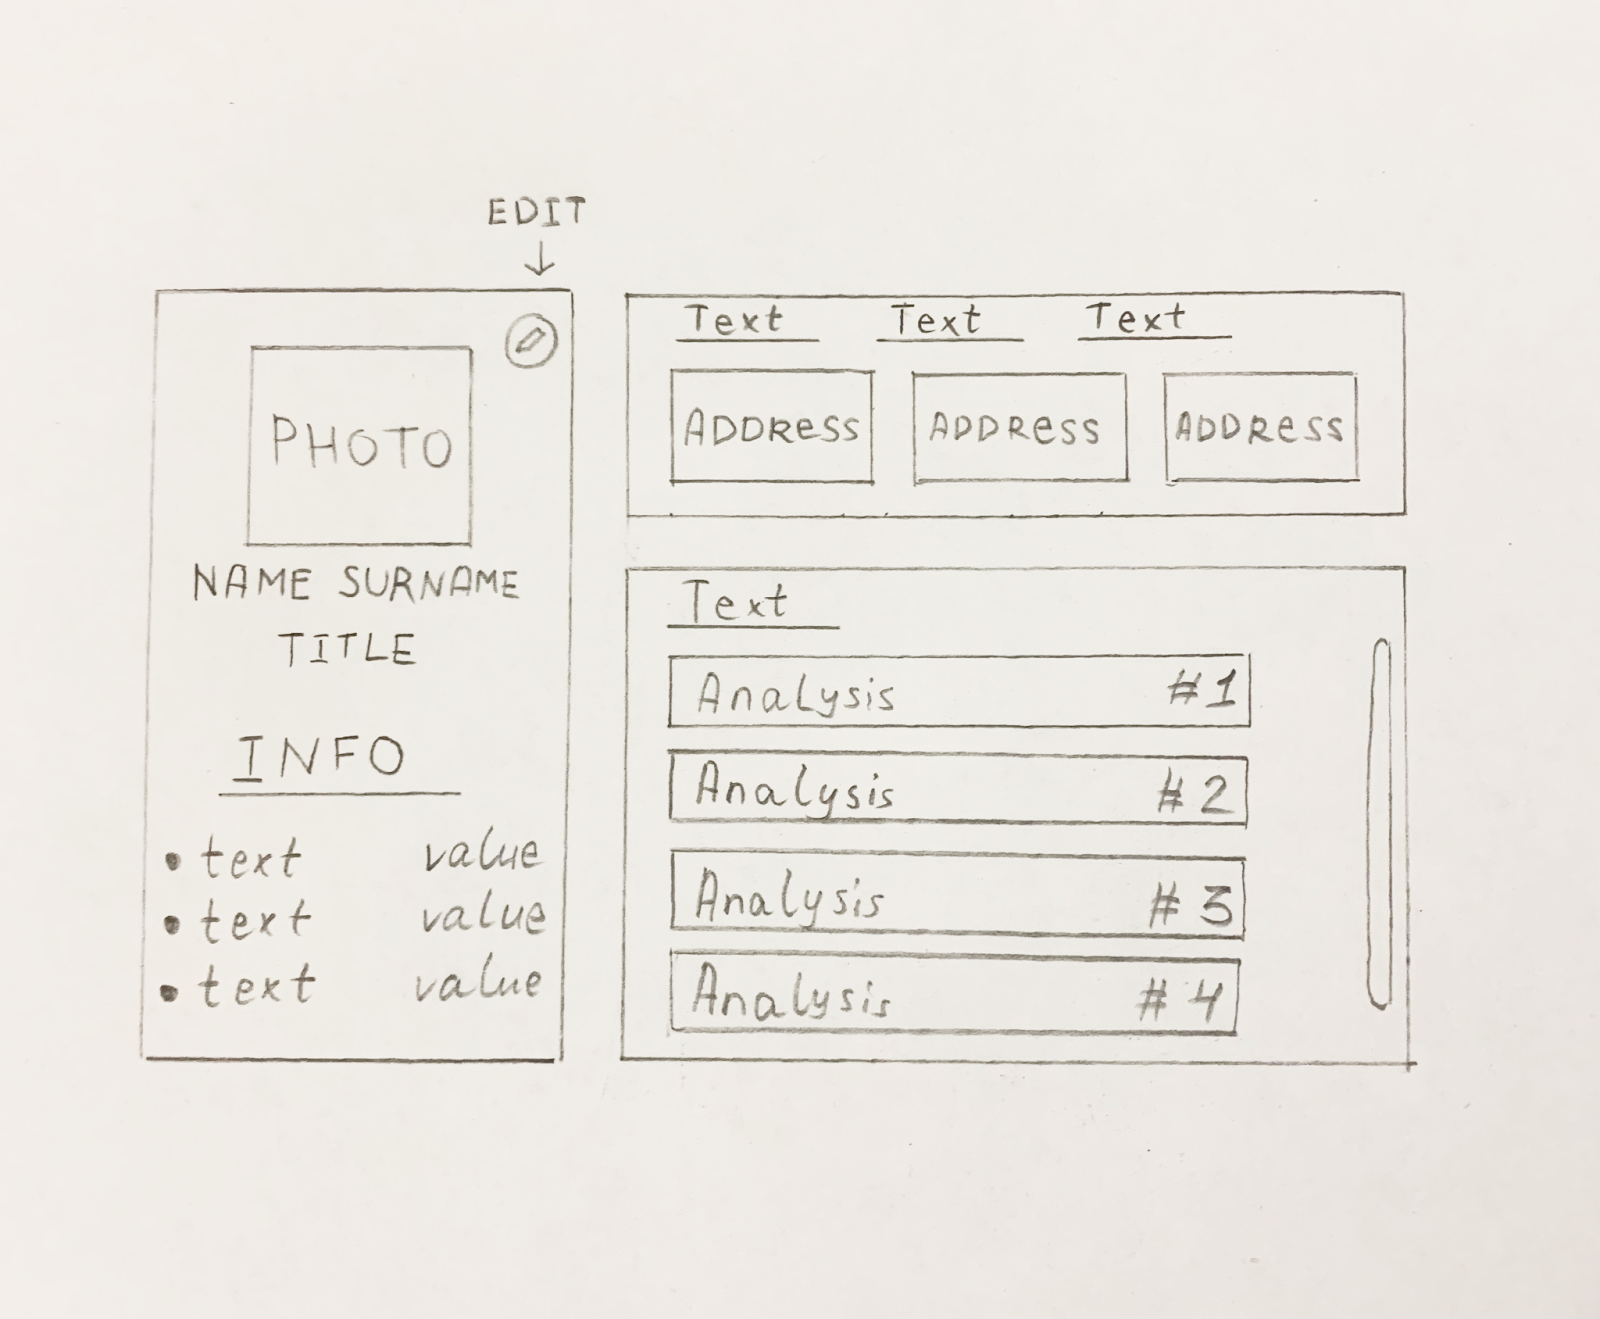
\includegraphics[scale=0.2]{figures/2.png}
    \caption{Sketch of the User profile}
    \label{fig:profilesketch}
\end{figure}
\par
The idea behind this profile page is to provide the user with unique information about them in one place. This page has several navigation that is different from the information that a regular unauthorized client owns. The sketch shows the initial ideas such as profile information on the side and information containers. The latest update will include tests and blood donation records. The purpose of a location with information about the profile is explained by the fact that it was necessary to make it larger for good visibility and on the left, since the user entering the page sees the elements on the left at the beginning. The information can change depending on the user. If you wish, you can change information about yourself by clicking on the edit button.

\section{Implementation of visual design and usability}
Usability testing made it possible to obtain information about how the user interacts with the site and, in general, to find out behavior. It took a long time to analyze user flows and  understand the importance of a completely new project design which doesn't have analogues. 
\par
After creating sketches and wireframes,it was necessary to start design scratches in order to implement the next part of the project, which is the design itself and its visualization. The value of visualization reveals the identity of the brand. For this, there were used the concepts and sketches prepared earlier. The visual implementation was changing several times so that the best practice for our product could be achieved. In Figma prototypes of the project is shown the process of the implementation, which demonstrates step by step changes depending on the user needs which were gathered throughout the project development.
\par
In general, the main goal is to create an interactive and user-friendly design with its own note of uniqueness for the donor project. The main tools of the designer helped in uniqueness. Coloristics, typography and fonts and interaction details were the most important aspects for us during the process of designing the website.

\section{Illustrations}
All illustrations that are on the pages are drawn by hand and they are also associated with blood. It was important not only to include unique content but to make it meaningful and eye-catching for the user, so that in future if some of our picture may be seen they will be immediately associated with the brand of 'Donor project'.
\par
An example of illustration shows test tubes with blood and a person sitting on the phone, showing us the mobility of the project and the interaction of medicine with technology. (see Figure \ref{fig:mainillustration})
\begin{figure}[h]
    \centering
    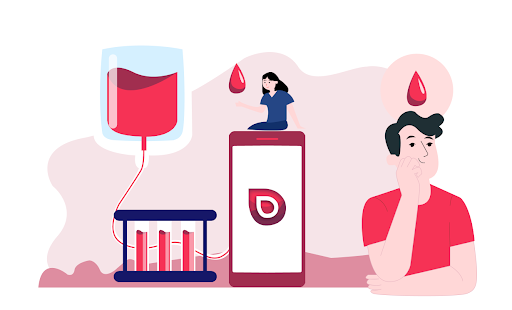
\includegraphics[scale=0.7]{figures/3.png}
    \caption{Illustration on the Main page}
    \label{fig:mainillustration}
\end{figure}

\section{Color scheme}
The goal is to create a simple, but at the same time to show in the design colorfulness and professionalism, expressed by confidence, emotions and even aroused desire among potential customers and users. 
\par
As we know, the donor project has a theme of medicine and blood, therefore, as studies of similar institutions and projects have shown, it is worth choosing colors associated with this area. Undoubtedly, the primary color was chosen for the page design is red. For a change, having played with the palette, we brought out several auxiliary colors. 
\par
The background itself is white for neutrality and visibility of key visual elements. The text received several shades: black, gray and shades of red. Black, white and gray are neutral colors. Neutral colors usually create a backdrop in design. They can be used on their own, or combined with another color accent. Black color was used for typography and other functional elements because of its neutrality. (see Figure \ref{fig:colorscheme})
\begin{figure}[h]
    \centering
    
\includegraphics[scale=0.5]{figures/4.png}
    \caption{Color Scheme}
    \label{fig:colorscheme}
\end{figure}
\par
White stands for purity and kindness. And the use of red is generally an art, since it is different and popping. It is the color of strength, so it can show irritability, anxiety, and even anger. But with the correct mixing of shades, in our case, frankness, love and confidence are shown.
The usage of white for the background and black for the text is a common technique that creates contrast between text and background and highlights other shades of elements on the site.

\section{Typography and fonts}
For the design there were used the fonts with good readability. The fonts do not contain additional elements, which can cause difficulties in recognizing the letters and slow down the speed of reading the text. Size of the font is big enough for comfortable reading. The font has no extra characters or serifs. Gilroy was chosen for the font. This font has twenty styles but its structure is very simple, therefore it is trendy today and fits well with design idea. (see Figure \ref{fig:font})
\par
As mentioned before in section of color significance, the text colors were based on black and shades of red. White and gray are used in dark places, there is no unreadable text in any place of the site, everywhere its own harmony. But black was replaced by dark red according to design measures. All this for easy reading and quick perception of the text. 
\par
\begin{figure}[h]
    \centering
    
\includegraphics[scale=0.5]{figures/5.png}
    \caption{Text-font example}
    \label{fig:font}
\end{figure}

\section{Interactive elements}
For the website version, we decided to add more motion and animations to attract the user. When swiping over the elements of the page, the user can see that most of the elements interact well with the user. Added animations, hovers on buttons, that is, they become moving and highlighted. On the main page, site visitors can see a slider with achievements that are also made by hand.
\begin{figure}[h]
    \centering
    
\includegraphics[scale=0.5]{figures/10.png}
    \caption{Buttons hover}
    \label{fig:buttons}
\end{figure}
\par
After logging in and viewing the achievements, illustrations were made with different logos of a certain achievement. Made in two styles to distinguish which achievements have been achieved and which have not yet been achieved. If there is a certain achievement, it will be filled and colored in red shades. 
\par
The uniqueness of the illustration also develop a habit of engagement in people's minds so that everything that is developed will be memorized by users. Aim was to be memorized, this will create strong association with the 'Donor project' and in future it will be much more easier to advertise the product.
\begin{figure}[h]
    \centering
    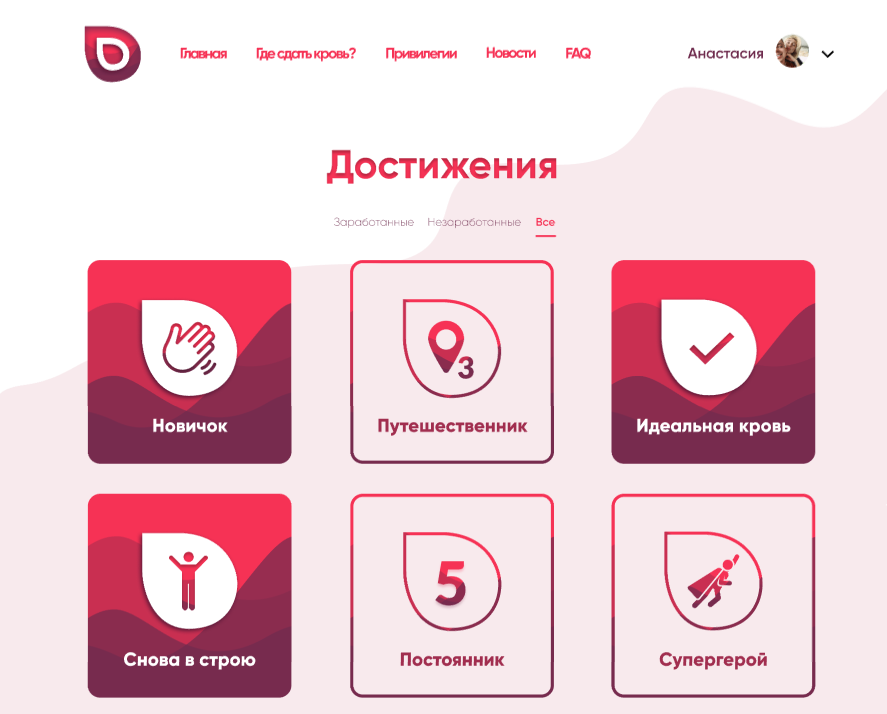
\includegraphics[scale=0.45]{figures/11.png}
    \caption{Text-font example}
    \label{fig:interactive}
\end{figure}





    \chapter{Marketing startegies}\label{ch:B}

\section{Social Media Marketing (SMM) in Donor project}
SMM currently transcends all boundaries and continues to play an important role in human life, all people have social networks where they spend most of their time \cite{macarthy}. They provide a single platform for companies to keep in touch with their customers and offer themselves or their product \cite{macarthy}.
\par
The number of social networks continues to grow in the world, and each of them has integration that helps to promote a particular business company in which the users themselves are interested. Therefore, developing companies strive for advertising promotions and SMM itself. Someone may say that this is the future prosperity of companies and we agreed with this statement and decided to use this in our project.
\par
Taking such steps as creating posts in the SMM format, we are preparing a skeleton of what we are and showing a novelty for some people. So by building the brand, preparing the website, we went to build a community around the brand to increase our loyal customer base.(see Figure \ref{fig:storyscreenshot})
\begin{figure}[h]
    \centering
    
\includegraphics[scale=0.7]{figures/6.jpeg}
    \caption{Instagram Story screenshot}
    \label{fig:storyscreenshot}
\end{figure}

\par
Before all this, what was said above, having familiarized ourselves with some sources, we came across advice to analyze the market in demand and need. We started this with the demand step. First of all Instagram stories went into action with a survey and helped to analyze the market as we said earlier. 

\section{Target and promotions online}

\par
After analyzing such types of stories in Instagram, this gave us several dozen responses, people were ready to help and there were a lot of donors. A lot of people had a feedback on such publication, but among them there were people who wanted to help but did not know how it all works, people who do not have enough information about donation. Thanks to this, we concluded that this project has a demand, so we decided to move on by launching a target page. 
\par
Targeting is a good option for a promotion, especially it is good for the 'Donor project', because it is an online platform and most of the user will definitely come from social media.
To target our potential donors, we created a new account on Instagram and began to promote it through stories, posts of friends, and then completely through the target. (see Figure \ref{fig:igaccount})
\begin{figure}[h]
    \centering
    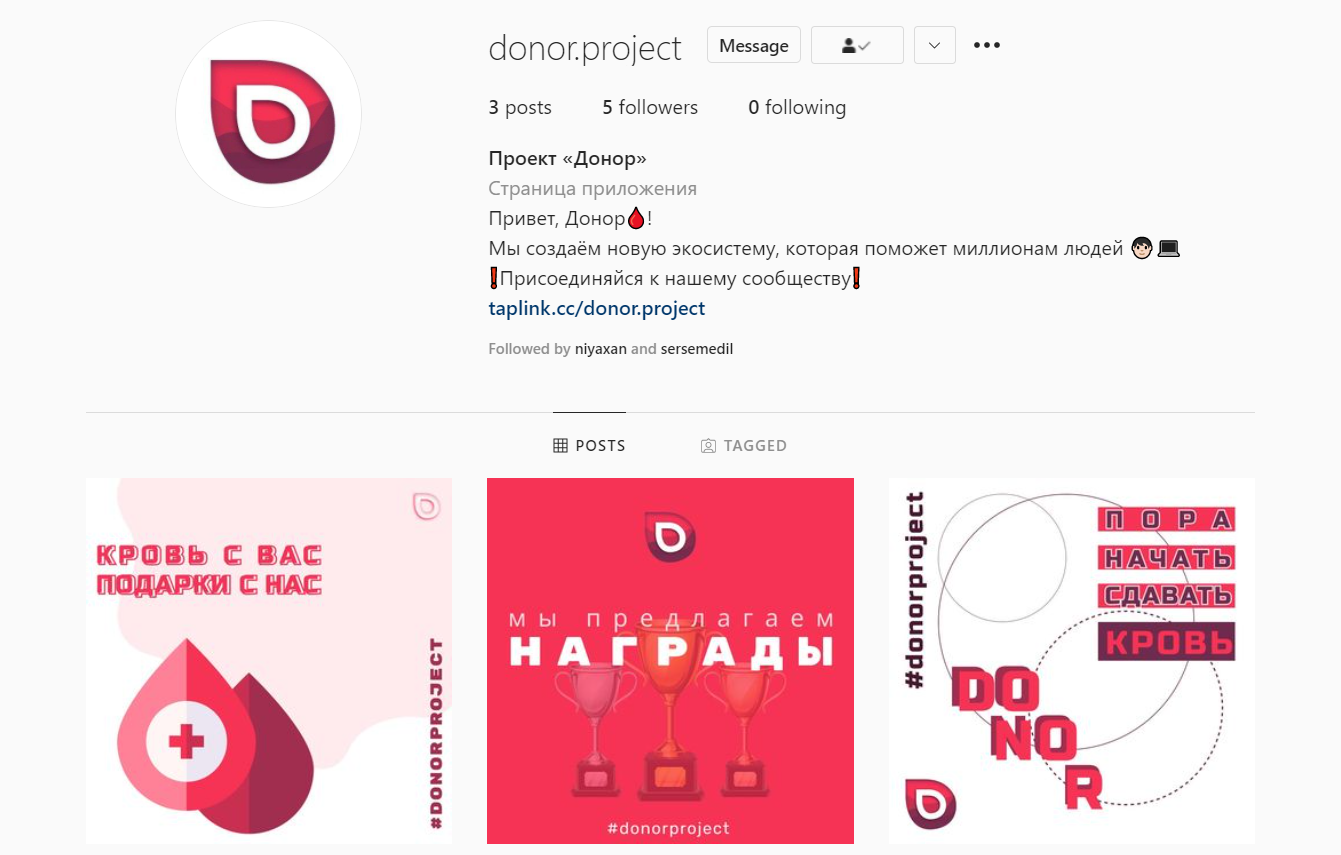
\includegraphics[scale=0.25]{figures/7.png}
    \caption{Instagram Profile of Donor project}
    \label{fig:igaccount}
\end{figure}
\par
To begin with, we went to the Facebook ads manager and set up everything that was needed for promotion. We posted a target, it was moderated and started working. Thus, they called and explained enlightened people in our project, indicating a link to our account intended for redirecting to a website. In our humble way, doing this business, that is, enlightenment, we think that we are helping to make this world a better place.
The Instagram account will also be entered by us. Our main logo was added to the branding of the account, which we put in the avatar. Also, to explain what we are, we threw a few posts with an explanation. After working in Figma, we made illustrations for posts.

\section{Award system and Integration}
Awards and privileges are a collection system for donating blood. On our site there is a separate page with all the possible bonuses that you can get and the prices next to it. Though the prices are indicated not in money, but in the campaigns of the blood donation. Prices are indicated in the site accumulation system and for each donation of blood you are credited with a certain number of bonuses. 
\par
Thus, having some points on your intra-site balance, you can purchase the bonuses that are available and provided by our program. Everyone can get acquainted with this on the page. If there are enough points on your account, you are asked to purchase one of the services to choose from. You buy some of the services if everything is correct and approved for you and you have a balance suitable for success. You can see more details on how many points you need under each bonus card that is provided on the website.
(see Figure \ref{fig:bonuses})

\begin{figure}[h]
    \centering
    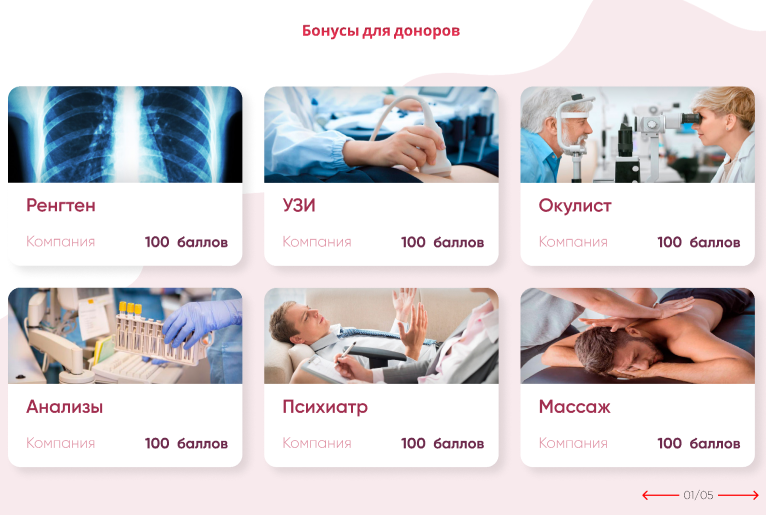
\includegraphics[scale=0.5]{figures/8.png}
    \caption{Bonus page of Donor project}
    \label{fig:bonuses}
\end{figure}
\par
As the statistics of visits has shown, this will be useful not only for our clients, but also for medical institutions. The donor donates blood by receiving bonuses, he goes to receive bonuses by choosing a medical institution. Receives a bonus, satisfaction, and on a subconscious level, the donor wants to return to the place where he received the bonus. 
\par
That is, we want to say that an ordinary user gets a profit from donating blood in exchange for receiving bonuses, and on the other hand, these hospitals where they provide services find new customers through our system. Thus, the two sides satisfy human and monetary needs.

\section{Badges of activity}
The main important thing of an online platform is to provide user ability of entertainment \cite{macarthy}. As we don't promote ourselves as an official presence such as news portal or governmental project, the idea of awarding developed through the process of working on the project. 
\par
System of awarding people with badges creates strong connection between simple user \cite{eyal}. As the researches show, people want to belong to a community and share ideas and thoughts that correlate with their own mind. Badge system was developed in order to prioritize layer of donors, so that new users will have a motivation not only to donate blood, but also receive some kind of appreciation of them in our system.
\par
There are special achievements for users, just like in games. These are not bonuses, this is a separate page on the site where various achievements are displayed and in order to complete them a user needs to complete blood donation history, depending on the number of blood donations and time. To open any achievement, user needs to follow your instructions in the description of the achievements.
\par
This will not only be interesting a user itself, but it will attract his friends and relatives, because, as the research shows, people are always trying to compete in different possible areas \cite{eyal}. And such competition as blood donation and enormous help to people in need is the best application.
(see Figure \ref{fig:achievements})

\begin{figure}[h]
    \centering
    
\includegraphics[scale=0.4]{figures/9.png}
    \caption{Achievements in Donor project}
    \label{fig:achievements}
\end{figure}
    \chapter{Physical Development of Donation System}\label{ch:C}
\section{Overview of the idea}
As the design system and implementation of the project went parallel, the changes from one to another were made accordingly. However only frontend part was similar to the design project that was stated at the beginning. 
\par
Main problem of the interaction is understanding between two opposite sides, it's a big work on developing user interface part, because in some cases there is no ability to show people the same web-site as it was established at the beginning. 'Donor project' website was done in the most simple way possible - HTML+CSS+JavaScript. In addition the usage of framework Jinja2 helped to avoid code repetition and code overlapping, so this technology was used fully in this project.
\par
Backend part in the process of the development wasn't affected as much as frontend. This is because the information coming had slightly changed. The simplicity of using Flask as a backend service allowed to develop lightweight system, that doesn't require much storage and memory space. In general, Python3 language was optimal solution for the project, because in future scaling we can easily perform on a big amount of data and users as well as we do on a small amount.
\par
Originally Django was chosen as a framework to implement backend. But as we began working with Django, we have figured out, that a lot of functions and methods that there are in the framework we basically don't need. Flask has been positioning itself as a microservice framework. This was the perfect solution.
\par
Most of the development time was spent on creating logically correct and functioning database. As a database structure has to be normalized, the process of adapting data that we had to a form of a relational database was long. This is because there was a lot of data retrieval, deleting and adding different columns. But as we have our minimum value product, now the structure is perfectly fits in current system.

\section{Database development and maintaining}
Developing database is a process of constant brainstorming. There are a lot of methods of showing relationship between entities, but for this project we didn't have a lot of entities to connect and the database is simple. So the optimal solution of visual representation was showing relationships between entities in a table form.
\par
This method allows to visualize main tables that are used more often than others \cite{adrianne}, so whilst rewriting it, we have managed to normalize database faster and easier.
(see Figure \ref{fig:relations})
\par
As a database storing from the developer side using PostgreSQL v.12 was perfect solution. It has more complicated functionality which allows to maintain data fast and without a lot of editing inputs and outputs. PostgreSQL tries to conform with the SQL standard where such conformance does not contradict traditional features or could lead to poor architectural decisions \cite{postgresql}. Our goal was to develop logic and a strong base for further development, because when database is strictly organized, then there is no problems in further development.

\begin{figure}[h]
    \centering
    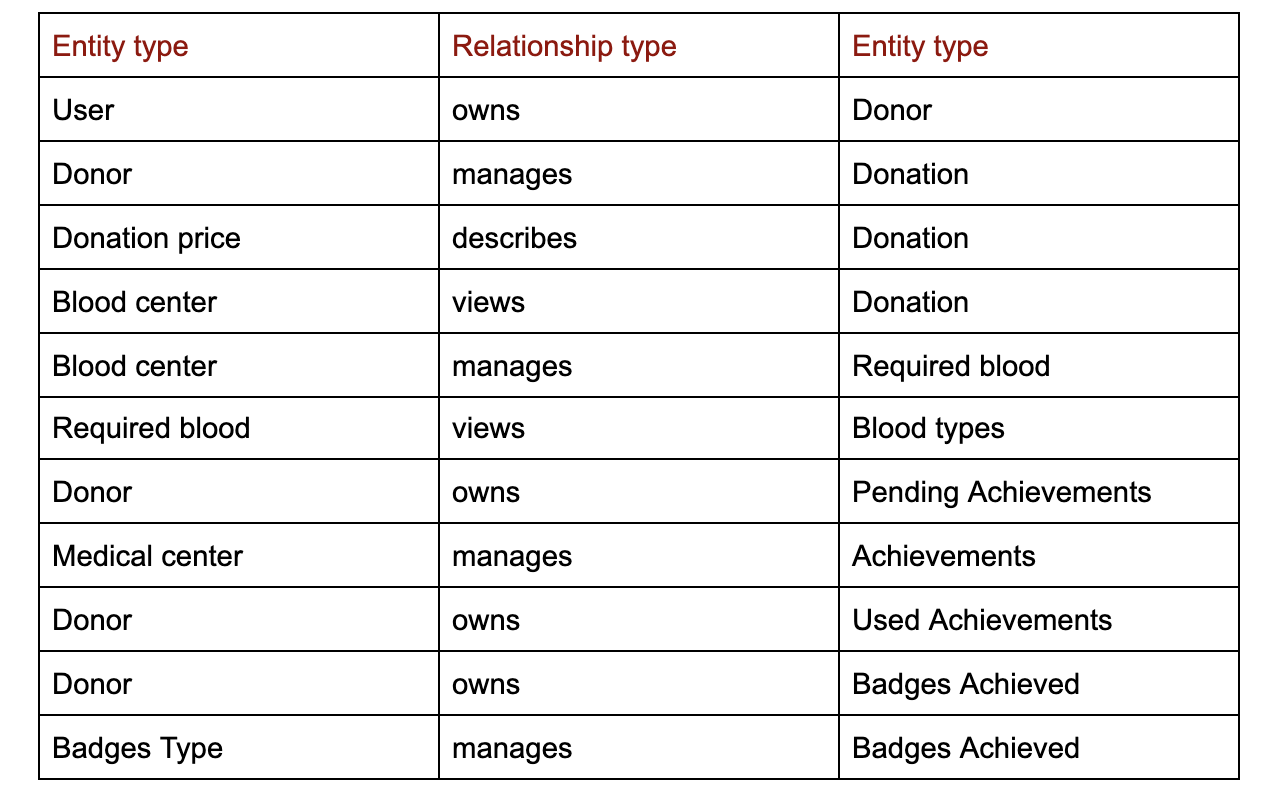
\includegraphics[scale=0.4]{figures/relations.png}
    \caption{Database table relations}
    \label{fig:relations}
\end{figure}

\section{Flask integration with PostgreSQL}
The connection between database and Flask doesn't require extra knowledge when both of the code structure and tables logic is organized. However there are some nuances that were used.
\par
\begin{lstlisting}

|-- Procfile
|-- app.py
|-- docker-compose.yml
|-- donorApp
|   |-- __init__.py
|   |-- donor.db
|   |-- helper_functions.py
|   |-- models.py
|   |-- routes.py
|   `-- templates

\end{lstlisting}

Flask application was structured in a different way, in order to simplify the view of each .py file. Main logic of all project configurations is stored in donorApp package. Basically everything that is related to database connection is stored as a configuration.

\begin{lstlisting}[language=Python]

app.config['SQLALCHEMY_DATABASE_URI'] =
'postgresql://<username>:<password>@localhost:<port>
/<database-name>'
app.config['SQLALCHEMY_TRACK_MODIFICATIONS'] = False
db = SQLAlchemy(app)

\end{lstlisting}
In order to manage the database the 'db' variable is used in main file of the project.
\par
Because SQLAlchemy is a common database abstraction layer and object relational mapper that requires a little bit of configuration effort, there is a Flask extension that handles that \cite{flasksql}.

\section{Docker-compose usage}
Quite often there are problems of implementing database packages on server-side. Also there might be difficulties in installing correct versions  and uninstalling unnecessary packages afterwards. So to avoid such consequences of running the project on broken database, docker-compose was chosen to maintain installation of the database package onto the server.
\par
The .yml file of the project is as simple as possible, because on this stage of the development we only use PostgreSQL. Docker calls the collection of files and instructions needed to run a software program an image \cite{docker}. 

\begin{lstlisting}[language=Python]

version: '3'
volumes:
  anketa_db_vol:

services:
  postgres:
    image: postgres:12
    volumes:
      - anketa_db_vol:/var/lib/postgresql/data
    environment:
      - POSTGRES_HOST=localhost
      - POSTGRES_PASSWORD=<password>
      - POSTGRES_DB=<database-name>
    ports:
      - "8432:5432"
    restart: always

\end{lstlisting}

\section{Backend implementation}
Architecture of Flask allowed fast and easy access to maintain, receive and publish data. The light structure demonstrates the code in the most simple way, so that even the developer who examines it for the first time will easily adapt to it. The example of the structure in the code snippet is a part of the project's method.

\begin{lstlisting}[language=Python]

@app.route('/logout', methods=['GET', 'POST'])
@login_required
def logout():
    logout_user()
    return redirect(url_for('main'))
    
\end{lstlisting}

\par
There is huge impact of the Flask database creation system. It allows to create entities without direct contact with database. This protects the structure and adds strict constraints in the development. So the ability to break tables or data stored is completely minimized.
\begin{lstlisting}[language=Python]
class User(db.Model, UserMixin):
    id = db.Column(db.Integer, primary_key=True)
    username = db.Column(db.String(80), unique=True)
    email = db.Column(db.String(120), unique=True)
    password = db.Column(db.String(120))
\end{lstlisting}
\par
It’s encouraged to use a package instead of a module for your flask application and drop the models into a separate module (Larger Applications) \cite{flasksql}.

\section{Frontend integration with Flask and Jinja2}
Jinja is a fast, expressive, extensible templating engine. Special placeholders in the template allow writing code similar to Python syntax \cite{jinja}.
Most common way to develop web-application on Python3 is to use this templating engine  to maintain frontend. 
\par
In 'Donor project' there are a lot of repeated blocks of code, which may be hard to follow, when the framework is not used. But when developing with Jinja2, it saves time and creates dynamic views, which don't require repeating. 
Also allowing to write code inside of the HTML code is huge advantage in frontend development. Whilst other frameworks like ReactJS require additional knowledge, Jinja offers common syntax that is perfect for small projects.
\begin{lstlisting}[language=HTML]





<!-- Preloader -->
<div id="page-loading-blocs-notifaction"></div>
<!-- Preloader END -->



\end{lstlisting}

Whilist developing front part there were a lot of changes from the original design that was made. This is justified by the functional requirements that were needed. 
\par
The interface of the web-design often doesn't have access to direct data that is being maintained from the user. In our case the development of the project started with the design idea and was followed by coding afterwards. Thus, we have common location of blocks, which doesn't break the original logic of wireframes, some of the design concept were not released in alpha-testing version.
\par
The concepts that haven't been used are following:
\begin{itemize}
  \item Main page detalized welcome image
  \item Representation of profile appointment scheduling
  \item The concept behind dropdown in header
\end{itemize}
\par
Though, those concept were not released, they were fully integrated into the system logically and have equivalent representation in 'Donor project' web-application.
    \chapter{Conclusion}\label{ch:concl}
\par
\section{Overview on the work done}
The result of the project development are:
\begin{itemize}
  \item Structured database, good developed connections between entities, logically correct relations between entities. Docker container allows to simplify the process of deployment.
  \item Beautiful website with simple user flow and functionality, which doesn't require a lot of skills to use. Points system is working perfectly.
  \item A good advertisement, SMM, Instagram development and attracting more younger people through social media.
\end{itemize}
\par
\section{Future development}
The main idea behind the 'Donor project' is make donation a common thing. Currently there is only blood donation in the system, but for the future development we are looking forward to integrate other donation types such as donation of bone marrow, sperm and women ovum donation. 

    

    \printbibliography[heading=bibintoc,title={References}]
\end{document}
